\section{Иллюстрация работы на модельных примерах}

Для наглядной демонстрации описанного подхода были построены унарные классификаторы для одного, двух и четырёх классов на модельных данных. В каждом случае в качестве фона использовались равномерно распределённые точки на единичном квадрате \([0, 1]^2\), а положительные объекты представляли собой выборки из компактных, хорошо различимых распределений.

На рисунке~\cref{fig:unary_one} показана граница принятия решения, построенная унарным классификатором для одного класса. Видно, что модель успешно выделяет область высокой плотности положительного класса, отсекая фон.

\begin{figure}[ht]
    \centerfloat{
        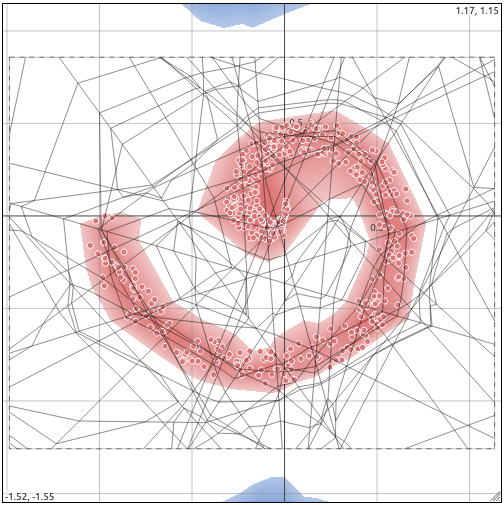
\includegraphics[width=0.9\linewidth]{Dissertation/images/ch2/usage/unary1.png}
    }
    \caption{Оценка плотности одного класса с использованием унарной схемы}
    \label{fig:unary_one}
\end{figure}

На рисунке~\cref{fig:unary_two} приведены результаты построения двух независимых унарных классификаторов для двух классов. Каждый классификатор определяет свою область плотности, и итоговая классификация осуществляется по наибольшей из двух аппроксимаций.

\begin{figure}[ht]
    \centerfloat{
        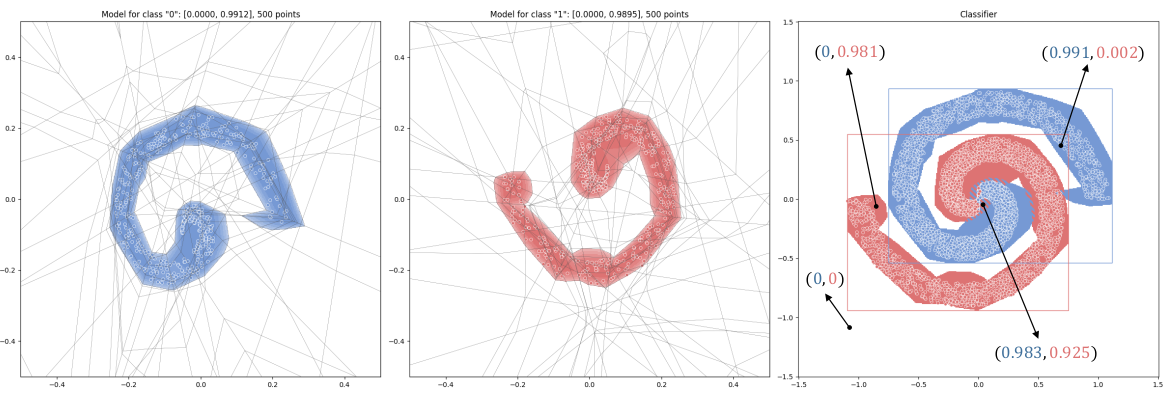
\includegraphics[width=\linewidth]{Dissertation/images/ch2/usage/unary2.png}
    }
    \caption{Унарная классификация для двух классов}
    \label{fig:unary_two}
\end{figure}

Наиболее показательный случай -- построение унарных классификаторов для четырёх классов с искусственно созданным дисбалансом. Один из классов содержит в семь раз больше наблюдений, чем другой, ещё один -- в пять раз больше и ещё один в три раза больше. Тем не менее, благодаря независимому обучению каждого классификатора на своём классе и фоновом множестве, области плотности получаются хорошо различимыми и не искаженными из-за дисбаланса. Это подтверждает устойчивость метода к нарушению пропорций классов (рисунок~\cref{fig:unary_four}).

\begin{figure}[ht]
    \centerfloat{
        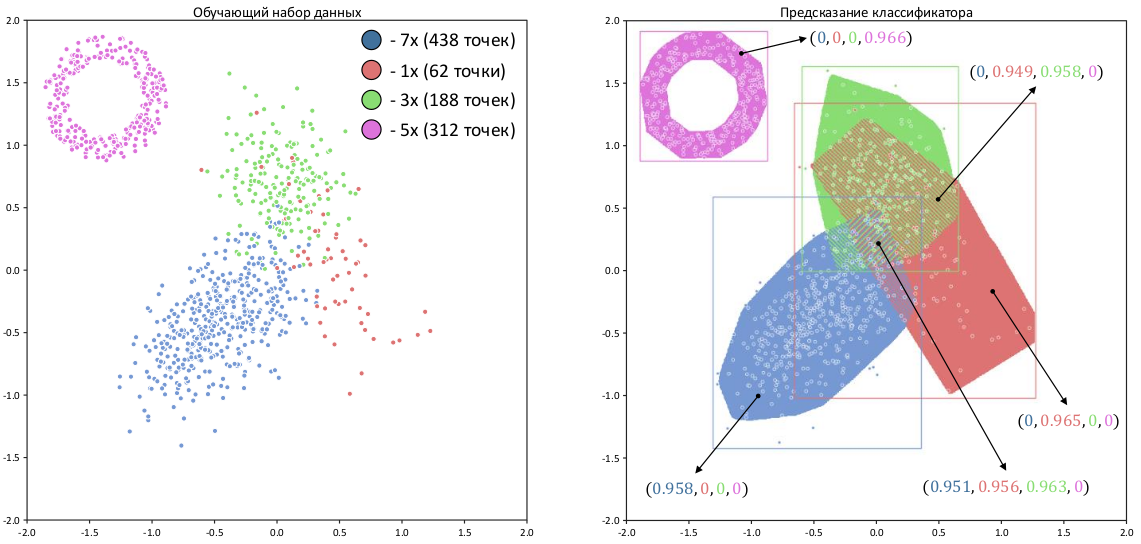
\includegraphics[width=\linewidth]{Dissertation/images/ch2/usage/unary4.png}
    }
    \caption{Унарная классификация для четырёх классов с дисбалансом}
    \label{fig:unary_four}
\end{figure}

Таким образом, предложенная схема построения унарных классификаторов позволяет надёжно и интерпретируемо решать задачу многоклассовой классификации, не требуя дополнительных допущений о балансе данных или единой архитектуре модели. Векторная оценка апостериорных вероятностей предоставляет дополнительную гибкость и возможность построения сложных решений с механизмами отказа или уточнения.